\chapter{背景知识}

% Sec 2.1
\section{LBM的起源}
格子玻尔兹曼方法起源于格子气自动机 (lattice gas automata, LGA) 方法。如方法中的名字所述,LBM继承了方法中格子的概念。LGA依赖于微观方法,在该方法中流体系统使用粒子描述,而非我们一般接触的宏观连续状态量。这些粒子在计算中并不能自由地无规则运动,而有一定的约束。在一个规则网格中,这些粒子只会在网格的相邻节点间\textit{迁移},并在格点发生\textit{碰撞}。在真实世界中,每次碰撞后粒子的速度应该是一个连续的独立变量,并可以先验得到。而因为格子的存在,速度空间只能被离散化,而不再是连续的空间。在一类LGA中,格子可能是六边形的,如图~\ref{img:LGA_lattice}所示,该类方法被称为FHP方法~\cite{frisch1986lattice},该方法根据三位提出者Frisch、Hasslacher与Pomeau命名。

\begin{figure}[htb]
    \centering
      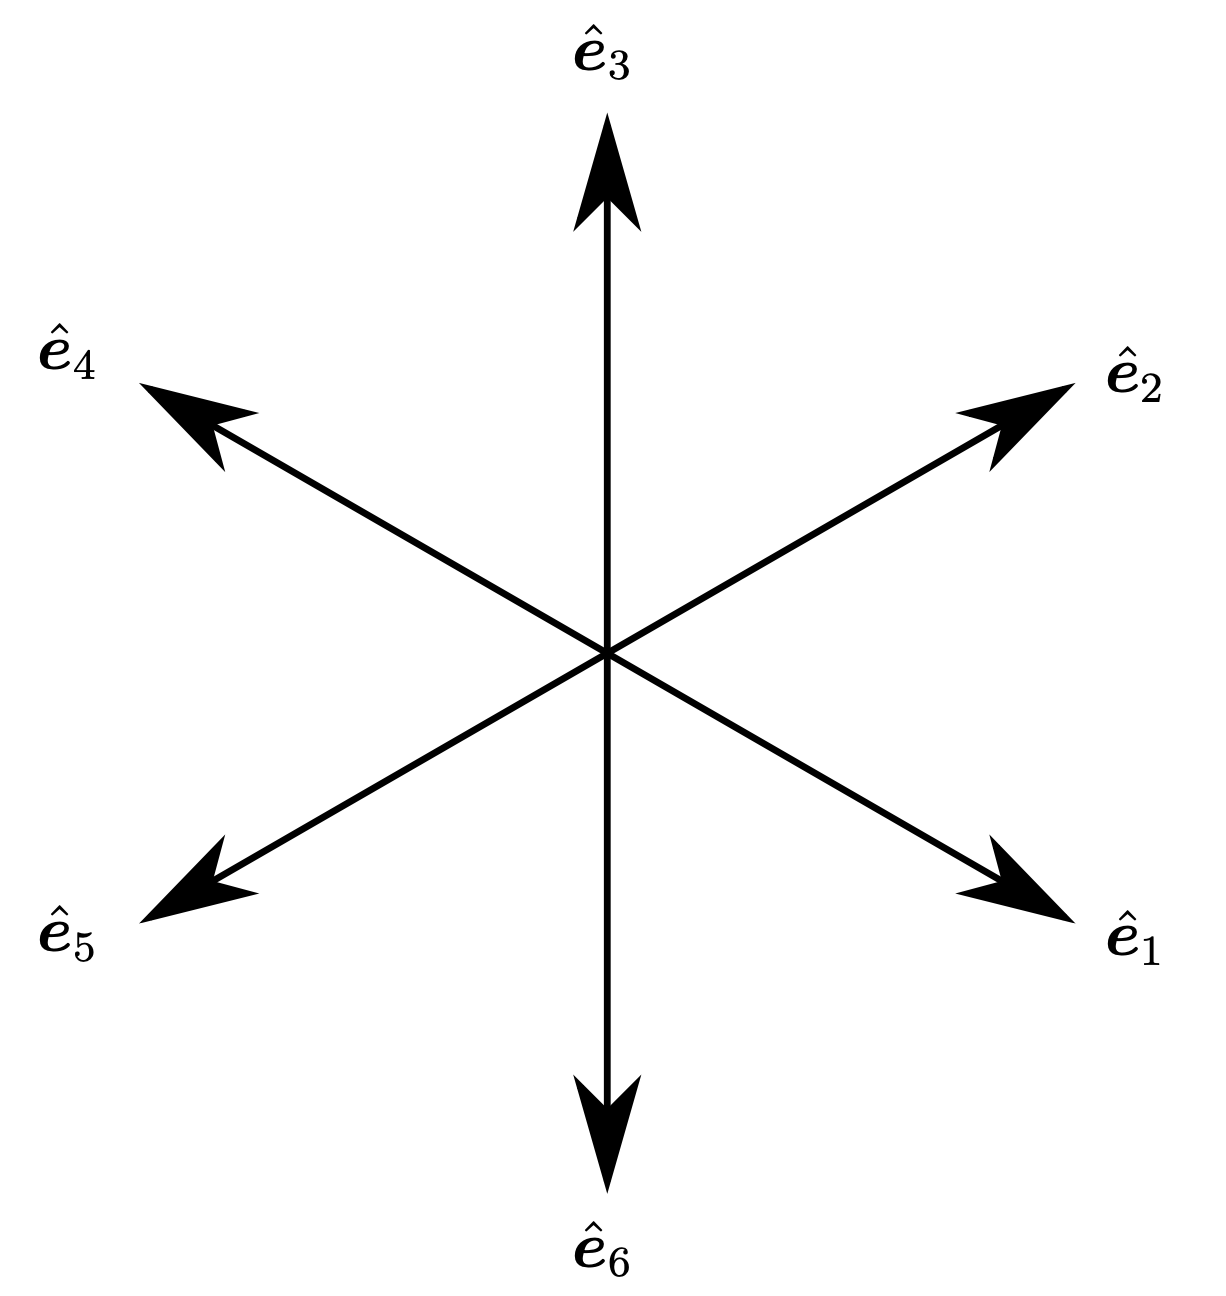
\includegraphics[width=0.5\columnwidth]{figures/LGA_lattice.png}
    \bicaption{\TODO{XXX}}{Hexagonial lattice of the FHP model with six discrete velocity directions in two-dimensional velocity space.}
    \label{img:LGA_lattice}
\end{figure}

不论LGA或LBM,有一个通用的假设是,在一个时间步长$\Delta t$后,一个粒子会正好走过两个相邻格点间的距离$\Delta x$。对于一个六边形网格,有
\begin{equation}
    \mathbf{\xi}_i=\frac{\Delta x}{\Delta t}\hat{\mathbf{e}}_i,
\end{equation}
其中$\hat{\mathbf{e}}_i=\mathbf{e}_i/|\mathbf{e}_i|$是正则化后的粒子运动方向,$i$是速度方向的标号,$\mathbf{\xi}_i$是离散速度。那么接下来可以定义粒子的状态$n_{i}(\mathbf{x},t)$,这个状态值可以是0或1。不考虑碰撞的话,粒子的运动可以用方程描述:
\begin{equation}
    n_{i}(\mathbf{x}+\mathbf{\xi}_i \Delta t,t+\Delta t)=n_{i}(\mathbf{x},t).
    \label{eq:LGA}
\end{equation}
公式~\ref{eq:LGA}构成了LGA中标志性的迁移步骤。这一过程也被LBM所继承。这一点为LBM方法带来了很大的优势,首先就是线性的对流项大幅降低了计算难度。其次是这一种直接的空间离散形式并不需要生成一个特殊的计算网格,使前处理的复杂度也能大幅下降。然而这并不代表LBM对网格完全没有要求,这类基于格子的方法只能被应用于六边形或更常见的笛卡尔网格也是一种对网格的约束。

在LGA中,因为粒子只有两种状态,所以经常使用布尔 (Boolean) 变量表示。一般值为真 (true) 时表示在某个空间位置上有一个粒子正在以特定的速度移动,而值为假 (false) 时表示没有这样的粒子。这清楚地显示LGA方法是在粒子层面来表示流体的运动的~\cite{wolf2004lattice}。而很显然,想要完全真实地使用粒子来表示流体是不现实的,因为$1cm^3$的空气中就含有约$2.7\times 10^{19}$个粒子。这导致LGA只能采用比现实情况要低得多的粒子量进行仿真,使结果有很强的噪声。从而方法需要在空间和时间上进行平均才能取得相对正常的结果。为了解决这一问题,McNamara和Zanetti~(\citeyear{mcnamara1988use})提出使用一个表示粒子密度的分布函数来替代这种单个的粒子。这种抽象的表达也是玻尔兹曼输运方程 (Boltzmann Transport Equation, BTE) 的构成基础。所以被传输的值不再只是一个布尔值,而是一个实数。这个实数表达了在空间位置$\mathbf{x}$、时间$t$,找到一个速度为$\mathbf{\xi}$的粒子的概率的空间密度。那么在没有碰撞时的迁移步骤的方程变为:
\begin{equation}
    f_{i}(\mathbf{x}+\mathbf{\xi}_i \Delta t,t+\Delta t)=f_{i}(\mathbf{x},t),
    \label{eq:LBM_streaming}
\end{equation}
其中$f_{i}$是上述的概率分布函数,一般简称为分布函数。一般认为这标志着LBM的诞生。因为在微观过程上使用了统计的概念,所以LBM被称为介观 (mesoscopic) 方法。在公式~\ref{eq:LGA}与~\ref{eq:LBM_streaming}中,粒子间的交互被忽略了。考虑粒子间的交互,这个过程可以表示为
\begin{equation}
    f_{i}(\mathbf{x}+\mathbf{\xi}_i \Delta t,t+\Delta t)=f_{i}(\mathbf{x},t)+\Omega(f_{i}(\mathbf{x},t)),
    \label{eq:LBM_in_one}
\end{equation}
其中$\Omega$是碰撞运算符。然而在实际中,通常会将公式~\ref{eq:LBM_in_one}表示为两个分开的过程,即碰撞和迁移:
\begin{alignat}{2}
\textbf{碰撞:} & \quad\quad &f_i^*(\boldsymbol{x}, t) & =f_i(\boldsymbol{x}, t)+\Omega\left(f_i(\boldsymbol{x}, t)\right); \\
\textbf{迁移:} & & f_i\left(\boldsymbol{x}+\boldsymbol{\xi}_i \Delta t, t+\Delta t\right) & =f_i^*(\boldsymbol{x}, t),
\end{alignat}
其中,$f_i^*$表示碰撞后的分布函数。为了满足质量与动量守恒,LGA中的碰撞中设定了一些固定的规则。对于FHP模型来说,其只允许两个或三个粒子间的碰撞,并且粒子离开格点的方向不能和进入格点的方向一样。这使得两个粒子间的碰撞只有两种可能的结果,而三个粒子间的碰撞只有一种可能的结果,参见图~\ref{img:LGA_collision}。

\begin{figure}[htb]
    \centering
      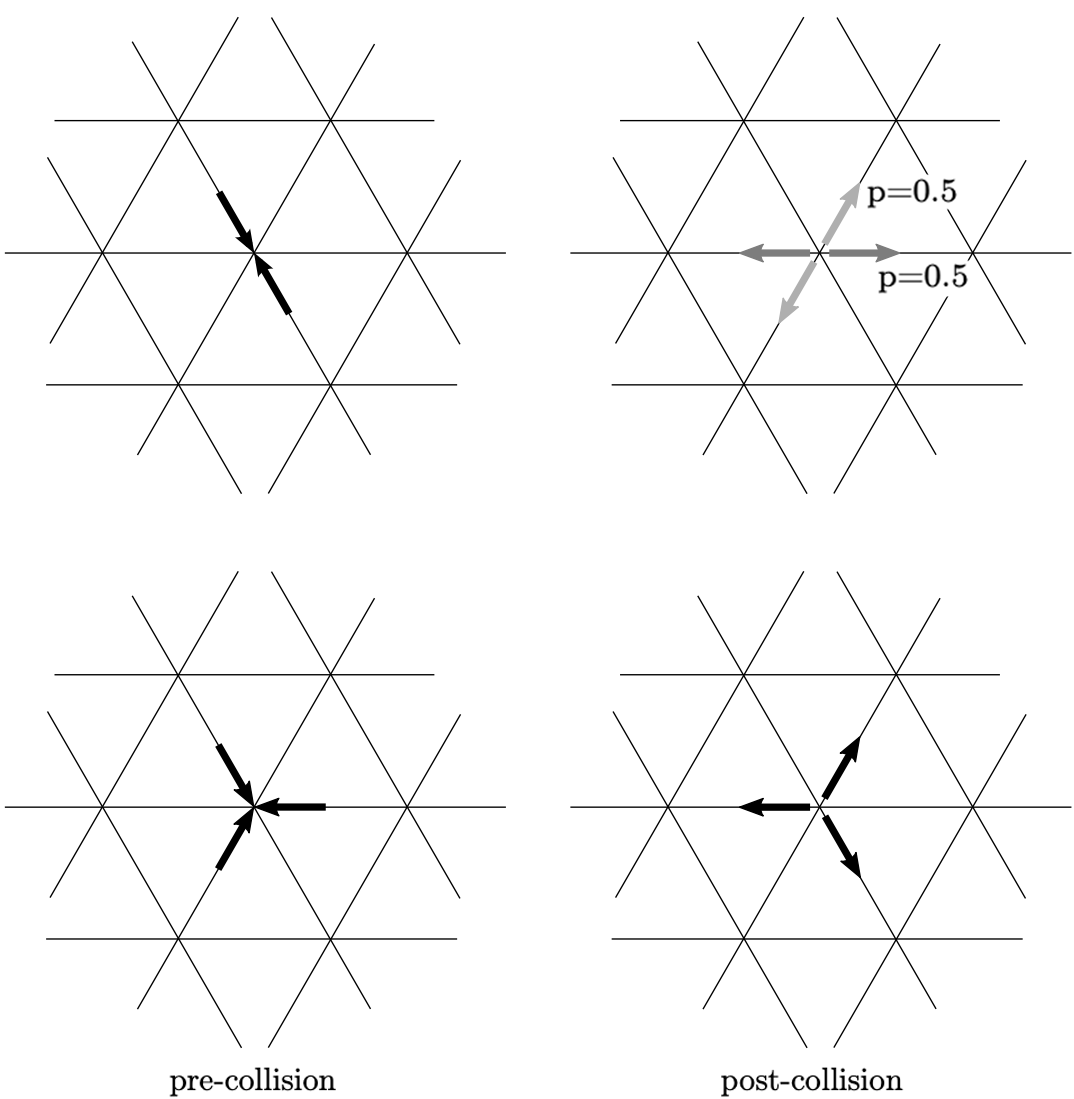
\includegraphics[width=0.9\columnwidth]{figures/LGA_collision.png}
    \bicaption{\TODO{XXX}}{Two- and three-particle collision in the FHP model. p denotes the probablility of a particular post-collision state.}
    \label{img:LGA_collision}
\end{figure}

虽然,最初的LB模型也是基于这些碰撞规则,但是很快人们发现这样的碰撞规则不仅物理上不够精确,对于三维来说,所需的计算量也是不现实的。于是另一种增强的碰撞方案被提出~\cite{higuera1989lattice, higuera1989boltzmann},该方案将非线性的碰撞运算进行了线性化,使碰撞后的值与一个平衡态产生联系:
\begin{equation}
    \Omega(f_{i}(\mathbf{x}, t))=\mathbf{A}_{\alpha\beta}(f_{i}(\mathbf{x},t)+f_{i}^{eq}(\mathbf{x},t)),
\end{equation}
其中$\mathbf{A}$是一个散射矩阵 (scattering matrix),$f_{i}^{eq}$是离散的麦克斯韦-玻尔兹曼平衡态函数 (Maxwell-Boltzmann equilibrium function)。之后Qian等~(\citeyear{qian1992lattice}) 进一步对碰撞模型的简化,基本确定了现在最常见的LBM的碰撞形式,即粒子间的碰撞可以看作是分布函数向平衡态的一个松弛过程:
\begin{equation}
    \mathbf{A}=-\delta_{\alpha\beta}\tilde{\omega}.
\end{equation}
那么这个散射矩阵事实上可以被一个松弛系数$\tilde{\omega}$替代了,这个系数是松弛时间$\tilde{\tau}$的倒数:$\tilde{\omega}^{-1}=\tilde{\tau}=\frac{\tau}{\Delta t}$. 从而,公式~\ref{eq:LBM_in_one}变为
\begin{equation}
    f_{i}(\mathbf{x}+\mathbf{\xi}_i \Delta t,t+\Delta t)=f_{i}(\mathbf{x},t)-\tilde{\omega}(f_{i}(\mathbf{x},t)-f_{i}^{eq}(\mathbf{x},t)).
    \label{eq:LBM_in_one_BGK}
\end{equation}
现在所有的分布函数都以相同的速率向平衡态松弛,虽然这样非常地简洁高效,但是这种方法没有考虑对于分布函数中有物理意义和没有意义的部分是否需要分开处理。之后d'Humières~(\citeyear{d1992generalized}) 证明散射矩阵$\mathbf{A}$可以由一组特征基得到,这为多松弛时间模型的出现奠定了基础。

这种对碰撞本身的效果建模,而不是对微观过程建模的想法,最早可见于连续玻尔兹曼方程中的BGK碰撞模型~\cite{Bhatnagar-1954}。这个想法背后的动机是碰撞过程的大部分细节并不会对宏观量产生影响,所以可以将这些过程省略。除了质量与动量守恒之外,BGK模型还满足$\mathrm{H}$-定理,即分布函数会向平衡态趋近。基于BGK的LBM也是最简洁、最常见的LBM模型。


% Sec 2.2
\section{从介观量到宏观量}
对于大多数的流体应用,使用一组连续的状态量来描述,如速度、压力等一般已经足够。这些量其实是微观粒子状态的统计平均。在宏观上,流体可以被视为连续体并由N-S方程描述。然而LBM并非是一个宏观方法,而是介于微观与宏观之间的介观层面,如图~\ref{img:fluid_abstraction}所示。

\begin{figure}[htb]
    \centering
      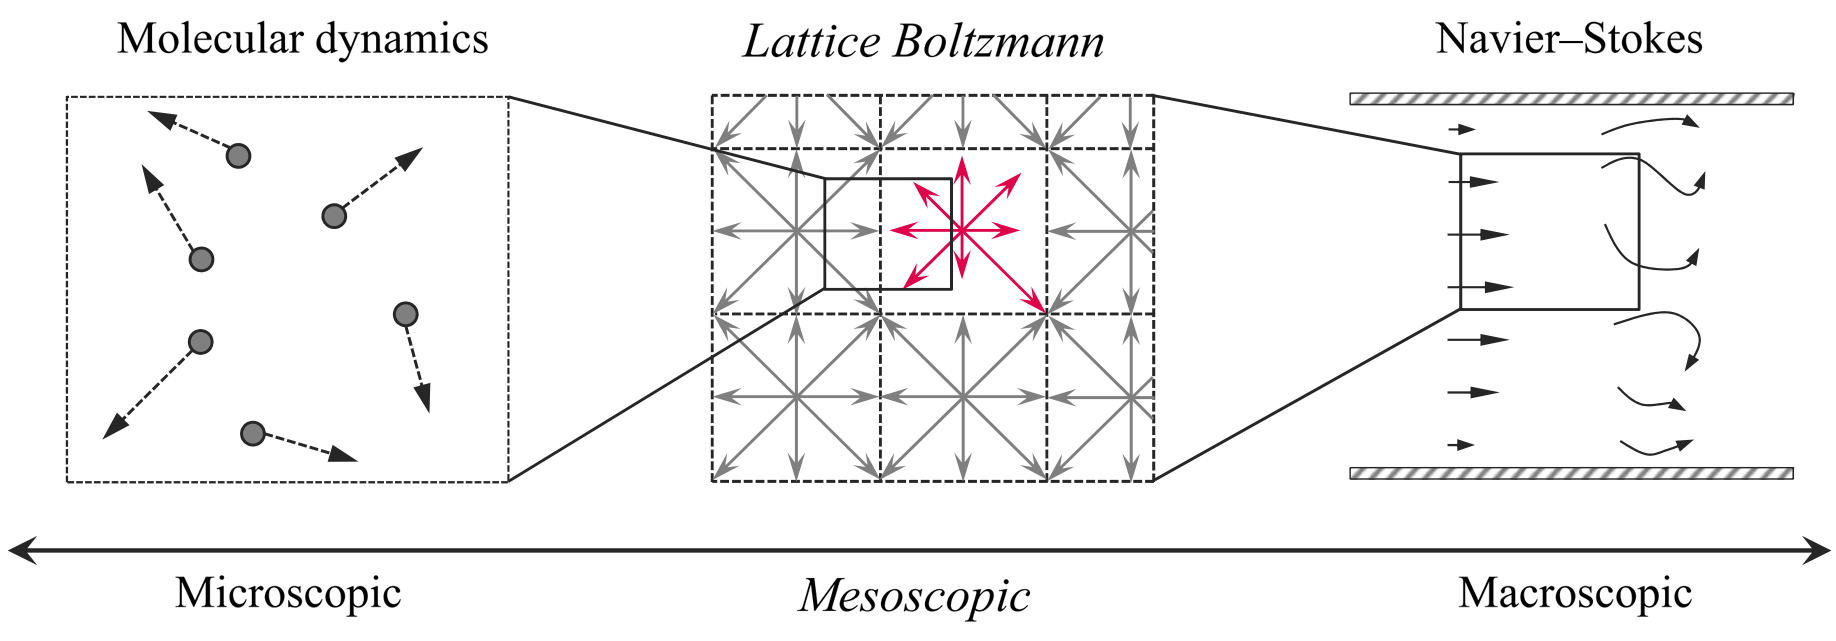
\includegraphics[width=0.9\columnwidth]{figures/fluid_abstraction.png}
    \bicaption{\TODO{XXX}}{Different abstraction levels of the fluid dynamics.}
    \label{img:fluid_abstraction}
\end{figure}

可以认为LBM虽然采用了一种非常简化的方案,但它依然计算了部分的微观层面的交互。这也使得LBM的求解过程与N-S方程求解有本质的区别。然而我们最终目的依然是获取宏观的流体状态,以符合我们在宏观世界中对流体的感受。接下来我们将逐步介绍LBM中的概念,并建立其与宏观世界的联系。

可以认为,在一个给定的控制体积 (control volume) 中,分布函数表示了速度在$\boldsymbol{\xi}$与$\boldsymbol{\xi}+d\boldsymbol{\xi}$之间的粒子总数。所以宏观和介观值可以通过对速度空间$\boldsymbol{Xi}$积分来建立,通过积分我们可以得到速度的n阶矩
\begin{equation}
    \boldsymbol{M}^{(n)}=\int_{\mathbb{R}^{\mathrm{D}}} \underbrace{\boldsymbol{\xi} \boldsymbol{\xi} \ldots \boldsymbol{\xi}}_{\mathrm{n} \text {次}} f(\boldsymbol{x}, \boldsymbol{\xi}, t) \mathrm{d} \boldsymbol{\xi},
\end{equation}
这里$D$代表积分的维度。在宏观层面,质量、动量和能量的守恒是由方程自身保证的,然而在介观层面,这些量的守恒需要由碰撞运算符保证,即
\begin{equation}
    \int\left(\Omega(f) \cdot \psi\right) \mathrm{d} \boldsymbol{\xi}=0,
    \label{eq:collision_invariants}
\end{equation}
其中$\psi_k$是碰撞不变量 (collision invariants),也就是可以令公式~\ref{eq:collision_invariants}成立的变量。可以证明,当$\psi=1, \boldsymbol{\xi}, |\boldsymbol{\xi}|^2$时,公式~\ref{eq:collision_invariants}是成立的。如果我们将碰撞不变量与分布函数的积进行积分,我们可以自然地得到连续速度空间中的宏观量
\begin{equation}
    \left\{\begin{array}{l}\rho(\boldsymbol{x}, t)=\int f(\boldsymbol{x}, \boldsymbol{\xi}, t) \mathrm{d} \boldsymbol{\xi} \\ \rho \boldsymbol{u}(\boldsymbol{x}, t)=\int \boldsymbol{\xi} f(\boldsymbol{x}, \boldsymbol{\xi}, t) \mathrm{d} \boldsymbol{\xi} \\ \rho E(\boldsymbol{x}, t)=\frac{1}{2} \int|\boldsymbol{\xi}|^2 f(\boldsymbol{x}, \boldsymbol{\xi}, t) \mathrm{d} \boldsymbol{\xi}\end{array}\right.,
\end{equation}
其中$E$为比能量 (specific energy)。对于单原子气体,碰撞可以假设为弹性的,所以比能量包含内能与动能
\begin{equation}
    \rho E=\rho\left(e+\frac{1}{2}|\boldsymbol{u}|^2\right).
\end{equation}
对于本动速度 (peculiar velocity) $\boldsymbol{v}=\boldsymbol{\xi}-\boldsymbol{u}$,即粒子在速度为$\boldsymbol{u}$的平均流中的相对速度,我们可以得到类似的能量守恒定律:
\begin{equation}
    \rho e(\boldsymbol{x}, t)=\frac{1}{2} \int|\boldsymbol{v}|^2 f(\boldsymbol{x}, \boldsymbol{\xi}, t) \mathrm{d} \boldsymbol{\xi}.
\end{equation}
在连续概念的流体力学中,内能的守恒方程需要通过一个状态方程$p=p(\rho,e)$将压力和密度联系起来,即
\begin{equation}
    p=\frac{1}{\mathrm{D}} \int|\boldsymbol{v}|^2 f(\boldsymbol{x}, \boldsymbol{\xi}, t) \mathrm{d} \boldsymbol{\xi}=\frac{2}{\mathrm{D}} \rho e.
    \label{eq:eos}
\end{equation}
对于满足理想气体定律 (perfect gas law) 的等温流体,可以得到
\begin{equation}
    e=\frac{\mathrm{D}}{2} \frac{p}{\rho}=\frac{\mathrm{D}}{2} R T_0=\frac{\mathrm{D}}{2} \frac{k_B T_0}{m}=\frac{\mathrm{D}}{2} c_s^2,
\end{equation}
其中$T_0$和$c_s$分别表示常值的温度与声速。所以公式~\ref{eq:eos}可以被重写为
\begin{equation}
    p=\rho c_s^2,
\end{equation}
即绝热系数$\gamma=1$时的等熵状态方程~\cite{kundu2015fluid}。


% Sec 2.3
\section{速度空间的离散化}
如前文所述,由于在求解时保留了格子的概念,所以我们必须类似地对速度空间进行离散。因为分布函数$f$对于任意阶的矩均有贡献,所以对于$f$,应该有一个多项式的表达。分布函数事实上可以表达为Hermite多项式构成的无穷级数,变量为经过声速正则化后的速度空间$\tilde{\xi}=\xi/c_s$:
\begin{equation}
    f(\boldsymbol{x}, \boldsymbol{\xi}, t)=\frac{1}{c_s^{\mathrm{D}}} \omega(\tilde{\boldsymbol{\xi}}) \sum_{n=0}^{\infty} \frac{1}{n !} \boldsymbol{a}^{(n)}(\boldsymbol{x}, t) \mathscr{H}^{(n)}(\tilde{\boldsymbol{\xi}}),
    \label{eq:hermite_f}
\end{equation}
其中$\mathscr{H}^{(n)}$是$n$次多项式。Hermite多项式的一个特点是展开系数$\boldsymbol{a}^{(n)}$是$f$本身的速度矩~\cite{shan2006kinetic},权重函数$\omega$为
\begin{equation}
    \omega(\tilde{\boldsymbol{\xi}})=\frac{1}{(2 \pi)^{\mathrm{D} / 2}} \exp \left(-\tilde{\boldsymbol{\xi}}^2 / 2\right).
\end{equation}
当流体不受压力时,流体可以被一个平衡态函数描述。这只会出现在密度和速度在整个流体域中都是常值的情况下。此时的平衡态可由麦克斯韦分布函数描述
\begin{equation}
    f^{eq}=\frac{\rho}{\left(2 \pi c_s^2\right)^{\mathrm{D} / 2}} \exp \left(\frac{-(\boldsymbol{\xi}-\boldsymbol{u})^2}{2 c_s^2}\right),
    \label{eq:maxwell_eq}
\end{equation}
其中$\rho$和$\boldsymbol{u}$分别为宏观的密度和速度。我们可以将这个平衡态函数投影到基为Hermite多项式的空间,此时速度矩变为$\boldsymbol{a}^{eq,(n)}$:
\begin{equation}
    f^{eq}(\boldsymbol{x}, \boldsymbol{\xi}, t)=\frac{1}{c_s^{\mathrm{D}}} \omega(\tilde{\boldsymbol{\xi}}) \sum_{n=0}^{\infty} \frac{1}{n !} \boldsymbol{a}^{eq,(n)}(\boldsymbol{x}, t) \mathscr{H}^{(n)}(\tilde{\boldsymbol{\xi}}).
    \label{eq:maxwell_eq_hermite}
\end{equation}
对比公式~\ref{eq:maxwell_eq},我们可以注意到两式几乎有着相同的形式。事实上,$f^{eq}$还可表达为
\begin{equation}
    f^{eq}=\frac{\rho}{c_s^D}\omega(\tilde{\boldsymbol{v}}),
\end{equation}
其中$\tilde{\boldsymbol{v}}=(\boldsymbol{\xi})$可视为本动马赫数。所以麦克斯韦分布函数的Hermite展开系数为
\begin{equation}
    \boldsymbol{a}^{eq,(n)}=\rho \int w(\tilde{\boldsymbol{v}}) \mathscr{H}^{(n)}\left(\tilde{\boldsymbol{v}}+\frac{\boldsymbol{u}}{c_s}\right) \mathrm{d} \tilde{\boldsymbol{v}}.
    \label{eq:hermite_coefficients}
\end{equation}
对公式~\ref{eq:hermite_f}这样的无穷级数进行截断,即对应着对速度空间的离散化,并且保证了连续空间和离散空间下的矩在截断的阶数前是不变的。而离散的一个重要约束来自于高斯积分
\begin{equation}
    \int w(\boldsymbol{x}) f(\boldsymbol{x}) \mathrm{d} \boldsymbol{x} \approx \sum w_i f\left(\boldsymbol{x}_i\right) \quad \text{with} \quad i=0,1, \ldots, q-1
\end{equation}
其中,$f(\boldsymbol{x})$可表示任意函数而$\omega_i$是常值的权重。
%我们用$\tilde{\xi}_i$表达在$N$阶截断后的Hermite级数的横坐标 (abscissae),则高阶的截断一定会需要更多数量的离散速度,使格子的拓扑更难构造。
则高斯积分的公式$E$可被抽象地记为
\begin{equation}
    E^q_{D,n},
\end{equation}
其中$D$表示空间的维度,$n$为积分精度的阶数,$q$表示积分所需要的点的数量。则我们可以推导出这三个值间的关系。对于一维空间,约束为$n>2N$并且$n=2q-1$~\cite{shan2006kinetic},即$q=N+1$。对于高维空间并没有一般的高斯积分理论,但是我们可以假设有
\begin{equation}
    q=(N+1)^D.
\end{equation}
则二维的速度空间在$N=2$阶截断时需要9个离散速度,$N=3$时需要16个。当然实际的格子方向可能有所不同,因为考虑到某些矩的对称性,在维持$N$不变时所需的离散速度数量可能会减少。然而从几何上考虑,要设计能充满空间且各向同性的格子可能又会增加所需的格子方向数量。如果依然采用~\cite{qian1992lattice}中的D$d$Q$q$的命名的话,能维持二阶精度的格子分别为D1Q3、D2Q9、D3Q16。由公式~\ref{eq:hermite_coefficients}可得,在截断至二阶时,Hermite展开的系数为
\begin{equation}
    \left\{\begin{array}{l}\boldsymbol{a}^{eq, 0}=\rho \\ \boldsymbol{a}^{eq, 1}=\rho \frac{\boldsymbol{u}}{c_0} \\ \boldsymbol{a}^{eq, 2}=\rho \frac{u_i u_j}{c_0^2}\end{array}\right.
\end{equation}
将其代入到公式~\ref{eq:maxwell_eq_hermite}中,可以得到
\begin{equation}
    f_i^{eq}(\boldsymbol{x}, t)=w_i \rho\left(1+\frac{\boldsymbol{\xi}_i \cdot \boldsymbol{u}}{c_0^2}+\frac{\left(\boldsymbol{\xi}_i \cdot \boldsymbol{u}\right)^2}{2 c_0^4}-\frac{u^2}{2 c_0^2}\right),
    \label{eq:f_eq_o2}
\end{equation}
其中$f_i^{eq}(\boldsymbol{x}, t)=f^{eq}(\boldsymbol{x}, \xi_i, t)$, $\omega_i=\omega(\frac{\xi}{c_s})/c_s^D$。上述的推导尝试用比较系统且严格的形式推导出分布函数及速度空间的离散,但同时尽量保持简洁,所以无法过于详尽地展示出所有步骤。对于更彻底的推导,读者们可以参考~\cite{shan2006kinetic, malaspinas2010lattice}。


% Sec 2.4
\section{从LBM到N-S方程}
在介绍过速度矩作为介观和宏观世界之间的联系之后,我们现在将使用多尺度分析 (Multiple-scale Analysis) 来从LBE推导出N-S方程。许多流体的动态特征其实表现于其与平衡态的偏移。如果在介观上,分布函数都处于平衡态,那么可以想像,在宏观上流体也是平静的。所以多尺度分析的思想是将$f$在$f^{eq}$处展开。展开后的$f^{eq}$可以被记为$f^{0}$,其余部分为非平衡态项:
\begin{equation}
    f=\underbrace{f^{(0)}}_{f^{e q}}+\underbrace{\epsilon f^{(1)}+\epsilon^2 f^{(2)}}_{f^{n e q}} \cdots .
\end{equation}
多尺度分析的扩展依赖于一个很小的参数$\epsilon$,这个值是碰撞时间$\tau=\nu/c_s^2$与格子时间步长$\Delta t$的比值。对流的时间尺度 (advection timescale) 是直接与$\Delta t_1=\tau/\epsilon$联系的,之后粘性扩散的时间尺度是联系于
\begin{equation}
    \Delta t_2=\frac{\Delta x^2}{\nu} \sim \frac{c_s^2 \Delta t^2}{\nu}=\frac{\tau}{\epsilon^2}
\end{equation}
的。有推导证明展开到一阶的$\epsilon$时,可以推导出欧拉方程~\cite{huang2008statistical}。展开到二阶时,时间上的导数为
\begin{equation}
    \frac{\partial}{\partial t}=\epsilon \frac{\partial}{\partial t_1}+\epsilon^2 \frac{\partial}{\partial t_2},
    \label{eq:ms_t}
\end{equation}
空间上的导数为
\begin{equation}
    \frac{\partial}{\partial \boldsymbol{x}}=\epsilon \frac{\partial}{\partial \boldsymbol{x}_1}.
    \label{eq:ms_x}
\end{equation}
在将$f$分解为平衡态与非平衡态后,公式~\ref{eq:collision_invariants}所表达的约束可被表达为
\begin{equation}
    \sum_{i} f_{i}^{(n)}=\sum_{i} \boldsymbol{\xi}_{i} f_{i}^{(n)}=0, \quad  n=1,2, \ldots.
\end{equation}
那么为了将LBE恢复到N-S方程,首先我们要将公式~\ref{eq:LBM_in_one_BGK}的左手侧进行二阶的泰勒展开
\begin{align}
    \begin{split}
        & f_{i}\left(\boldsymbol{x}+\boldsymbol{\xi}_{i} \Delta t, t+\Delta t\right) \approx \\
        & \quad f_{i}(\boldsymbol{x}, t)+\left(\xi_{i \alpha} \Delta t \frac{\partial}{\partial x_{\alpha}}+\Delta t \frac{\partial}{\partial t}\right) f_{i}(\boldsymbol{x}, t)+ \\
        & \quad \frac{1}{2}\left(\xi_{i \alpha} \xi_{i \beta} \Delta t^{2} \frac{\partial^{2}}{\partial x_{\alpha} \partial x_{\beta}}+2 \xi_{i \alpha} \Delta t^{2} \frac{\partial}{\partial x_{\alpha}} \frac{\partial}{\partial t}+\Delta t^{2} \frac{\partial^{2}}{\partial t^{2}}\right) f_{\alpha}(\boldsymbol{x}, t)+\mathcal{O}\left(\Delta t^{3}\right) .
    \end{split}
\end{align}
我们将上式代入公式~\ref{eq:LBM_in_one_BGK},并用$\tau$替代$\tilde{\omega}$后,可以得到
\begin{equation}
\Delta t\left(\xi_{i \alpha} \frac{\partial}{\partial x_{\alpha}}+\frac{\partial}{\partial t}\right) f_{\alpha}+\frac{\Delta t^{2}}{2}\left(\xi_{i \alpha} \xi_{i \beta} \frac{\partial^{2}}{\partial x_{\alpha} \partial x_{\beta}}+2 \xi_{i \alpha} \frac{\partial}{\partial x_{\alpha}} \frac{\partial}{\partial t}+\frac{\partial^{2}}{\partial t^{2}}\right) f_{\alpha}=-\frac{\Delta t}{\tau}\left(f_{\alpha}-f_{\alpha}^{e q}\right) .
\end{equation}
接下来,我们将多尺度分析的公式~\ref{eq:ms_t}与~\ref{eq:ms_x}代入
\begin{align}
    \begin{split}
& {\left[\xi_{\alpha i}\left(\epsilon \frac{\partial}{\partial x_{1 i}}\right)+\left(\epsilon \frac{\partial}{\partial t_{1}}+\epsilon^{2} \frac{\partial}{\partial t_{2}}\right)\right]\left(f_{\alpha}^{(0)}+\epsilon f_{\alpha}^{(1)}+\epsilon^{2} f_{\alpha}^{(2)}\right)+} \\
& \frac{\Delta t}{2}\left[\xi_{\alpha i} \xi_{\alpha j}\left(\epsilon^{2} \frac{\partial^{2}}{\partial x_{1 i} \partial x_{1 j}}\right)+\left(2 \xi_{\alpha i} \epsilon^{2} \frac{\partial}{\partial x_{1 i}} \frac{\partial}{\partial t_{1}}\right)+\left(\epsilon^{2} \frac{\partial^{2}}{\partial t_{1}^{2}}\right)\right]\left(f_{\alpha}^{(0)}+\epsilon f_{\alpha}^{(1)}+\epsilon^{2} f_{\alpha}^{(2)}\right)= \\
& \quad-\frac{1}{\tau}\left(f_{\alpha}^{(0)}+\epsilon f_{\alpha}^{(1)}+\epsilon^{2} f_{\alpha}^{(2)}-f_{\alpha}^{e q}\right) .
    \end{split}
    \label{eq:ms_total}
\end{align}
接下来,我们把公式~\ref{eq:ms_total}按照$\epsilon$的阶数分离:

\noindent
$\mathcal{O}\left(\epsilon^{0}\right):$
\begin{equation}
f_{\alpha}^{(0)}=f_{\alpha}^{e q}
\end{equation}
$\mathcal{O}\left(\epsilon^{1}\right):$
\begin{equation}
\epsilon\left(\xi_{\alpha i} \frac{\partial}{\partial x_{1 i}}+\frac{\partial}{\partial t_{1}}\right) f_{\alpha}^{(0)}=-\frac{1}{\tau} \epsilon f_{\alpha}^{(1)}
\label{eq:ms_o1}
\end{equation}
$\mathcal{O}\left(\epsilon^{2}\right):$
\begin{equation}
\epsilon^{2} \frac{\partial}{\partial t_{2}} f_{\alpha}^{(0)}+\left(\xi_{\alpha i} \epsilon \frac{\partial}{\partial x_{1 i}}+\epsilon \frac{\partial}{\partial t_{1}}\right) \epsilon f_{\alpha}^{(1)}+\frac{\Delta t}{2}\left(\xi_{\alpha i} \epsilon \frac{\partial}{\partial x_{1 i}}+\epsilon \frac{\partial}{\partial t_{1}}\right)^{2} f_{\alpha}^{(0)}=-\frac{1}{\tau} \epsilon^{2} f_{\alpha}^{(2)}
\label{eq:ms_o2}
\end{equation}
将公式~\ref{eq:ms_o1}代入公式~\ref{eq:ms_o2},可以得到
\begin{equation}
\epsilon^{2} \frac{\partial}{\partial t_{2}} f_{\alpha}^{(0)}+\left(\xi_{\alpha i} \epsilon \frac{\partial}{\partial x_{1 i}}+\epsilon \frac{\partial}{\partial t_{1}}\right)\left(1-\frac{\Delta t}{2 \tau}\right) \epsilon f_{\alpha}^{(1)}=-\frac{1}{\tau} \epsilon^{2} f_{\alpha}^{(2)}
\label{eq:ms_o1_into_o2}
\end{equation}
接下来我们想要获得关于宏观量的守恒公式,与求矩类似,我们对公式~\ref{eq:ms_o1}与公式~\ref{eq:ms_o1_into_o2}对碰撞不变量积分得到
\begin{equation}
\epsilon \frac{\partial \rho}{\partial t_{1}}+\epsilon \frac{\partial \rho u_{i}}{\partial x_{1 i}}=0,
\label{eq:ms_moment_o1_a}
\end{equation}
\begin{equation}
\epsilon \frac{\partial \rho u_{i}}{\partial t_{1}}+\epsilon \frac{\partial P_{i j}^{(0)}}{\partial x_{1 j}}=0,
\label{eq:ms_moment_o1_b}
\end{equation}
即无粘的欧拉公式。同样地,我们对公式~\ref{eq:ms_o2}积分得到
\begin{equation}
\epsilon^{2} \frac{\partial \rho}{\partial t_{2}} = 0,
\end{equation}
\begin{equation}
\epsilon^{2} \frac{\partial \rho u_{i}}{\partial t_{2}} +\left(1-\frac{\Delta t}{2 \tau}\right) \epsilon^{2} \frac{P_{i j}^{(1)}}{\partial x_{1 j}}=0 .
\end{equation}
然后我们将同阶数的部分归化到一起,可以得到0阶的矩方程
\begin{equation}
\frac{\partial \rho}{\partial t}+\frac{\partial \rho u_{i}}{\partial x_{i}}=0,
\end{equation}
即连续性方程。1阶的矩方程为
\begin{equation}
\frac{\partial \rho u_{i}}{\partial t}+\frac{\partial}{\partial x_{j}}\left[P_{i j}^{e q}+\left(1-\frac{\Delta t}{2 \tau}\right) P_{i j}^{n e q}\right]=0,
\end{equation}
为了计算$P_{i j}^{n e q}$,我们将公式~\ref{eq:ms_o1}转为二阶矩方程,得到
\begin{equation}
\epsilon \frac{\partial P_{i j}^{(0)}}{\partial t_{1}}+\epsilon \frac{\partial Q_{i j k}^{(0)}}{\partial x_{1 k}}=-\frac{1}{\tau} \epsilon P_{i j}^{(1)}.
\label{eq:ms_moment_o2}
\end{equation}
由公式~\ref{eq:f_eq_o2}我们可以由下面的方式得到三阶矩$Q_{ijk}$,
\begin{equation}
Q_{i j k}^{(0)}=Q_{i j k}^{e q}=\sum_{\alpha} f_{\alpha}^{e q} \xi_{\alpha, i} \xi_{\alpha, j} \xi_{\alpha, k}=\rho c_{0}^{2}\left(u_{i} \delta_{j k}+u_{j} \delta_{i k}+u_{k} \delta_{i j}\right).
\end{equation}
接下来,我们引入如下的积分公式 (乘积法则):
\begin{align}
\epsilon \frac{\partial \rho u_{i} u_{j}}{\partial t_{1}} & =u_{i} \epsilon \frac{\rho u_{j}}{\partial t_{1}}+u_{j} \epsilon \frac{\rho u_{i}}{\partial t_{1}}-u_{i} u_{j} \epsilon \frac{\partial \rho}{\partial t_{1}}, \\
\epsilon \frac{\partial \rho u_{i} u_{j} u_{k}}{\partial x_{1 k}} & =u_{i} \epsilon \frac{\rho u_{j} u_{k}}{\partial x_{1 k}}+u_{j} \epsilon \frac{\rho u_{i} u_{k}}{\partial x_{1 k}}-u_{i} u_{j} \epsilon \frac{\partial \rho u_{k}}{\partial x_{1 k}} .
\end{align}
使用上述的公式,公式~\ref{eq:ms_moment_o2}的左手边的$\epsilon \frac{\partial P_{i j}^{(0)}}{\partial t_{1}}$可以被表达为
\begin{align}
    \begin{split}
\epsilon \frac{\partial P_{i j}^{(0)}}{\partial t_{1}}= & \epsilon \frac{\partial \rho u_{i} u_{j}}{\partial t_{1}}+c_{0}^{2} \delta_{i j} \epsilon \frac{\partial \rho}{\partial t_{1}} \\
= & u_{i} \epsilon \frac{\partial \rho u_{j}}{\partial t_{1}}+u_{j} \epsilon \frac{\partial \rho u_{i}}{\partial t_{1}}-u_{i} u_{j} \epsilon \frac{\partial \rho}{\partial t_{1}}+c_{0}^{2} \delta_{i j} \epsilon \frac{\partial \rho}{\partial t_{1}} \\
= & -u_{i} \epsilon \frac{\partial P_{j k}^{(0)}}{\partial x_{1 k}}-u_{j} \epsilon \frac{\partial P_{i j}^{(0)}}{\partial x_{1 k}}+u_{i} u_{j} \epsilon \frac{\partial \rho u_{k}}{\partial x_{1 k}}-c_{0}^{2} \delta_{i j} \epsilon \frac{\partial \rho u_{k}}{\partial x_{1 k}} \quad \text {(由公式~\ref{eq:ms_moment_o1_a}、\ref{eq:ms_moment_o1_b})} \\
= & -u_{i} \epsilon \frac{\partial}{\partial x_{1 k}}\left(\rho u_{j} u_{k}+\rho c_{0}^{2} \delta_{j k}\right)-u_{j} \epsilon \frac{\partial}{\partial x_{1 k}}\left(\rho u_{i} u_{k}+\rho c_{0}^{2} \delta_{i k}\right) \\
& +u_{i} u_{j} \epsilon \frac{\partial \rho u_{k}}{\partial x_{1 k}}-c_{0}^{2} \delta_{i j} \frac{\partial \rho u_{k}}{\partial x_{1 k}} \\
= & -\epsilon \frac{\partial \rho u_{i} u_{j} u_{k}}{\partial x_{1 k}}-c_{0}^{2}\left(u_{i} \epsilon \frac{\partial \rho}{\partial x_{1 j}}+u_{j} \epsilon \frac{\partial \rho}{\partial x_{1 i}}\right)-c_{0}^{2} \delta_{i j} \epsilon \frac{\partial \rho u_{k}}{\partial x_{1 k}} .
    \end{split}
\end{align}
同时,$\epsilon \frac{\partial Q_{i j k}^{(0)}}{\partial x_{1 k}}$可表达为
\begin{align}
    \begin{split}
\epsilon \frac{\partial Q_{i j k}^{(0)}}{\partial x_{1 k}} & =\epsilon \frac{\partial}{\partial x_{1 k}} \rho c_{0}^{2}\left(u_{i} \delta_{j k}+u_{j} \delta_{i k}+u_{k} \delta_{i j}\right) \\
& =c_{0}^{2}\left(\epsilon \frac{\partial \rho u_{i}}{\partial x_{1 j}}+\epsilon \frac{\partial \rho u_{j}}{\partial x_{1 i}}\right)+c_{0}^{2} \delta_{i j} \epsilon \frac{\partial \rho u_{k}}{\partial x_{1 k}}.
    \end{split}
\end{align}
将上述两公式相加可得到$P_{i j}^{(1)}$的表达式
\begin{equation}
\epsilon P_{i j}^{(1)}=-\rho c_{0}^{2} \tau\left(\epsilon \frac{\partial u_{i}}{\partial x_{1 j}}+\epsilon \frac{\partial u_{j}}{\partial x_{1 i}}\right)+\tau \epsilon \frac{\partial \rho u_{i} u_{j} u_{k}}{\partial x_{1 k}}.
\end{equation}
将 $P^{n e q}=\epsilon P^{(1)}$,$\partial / \partial \boldsymbol{x}=\epsilon \partial / \partial \boldsymbol{x}_{1}$代入,我们可以获得
\begin{equation}
P_{i j}^{n e q}=\underbrace{-\rho c_{0}^{2} \tau\left(\frac{\partial u_{i}}{\partial x_{j}}+\frac{\partial u_{j}}{\partial x_{i}}\right)}_{\boldsymbol{\sigma}^{\prime}}+\underbrace{\tau \frac{\partial \rho u_{i} u_{j} u_{k}}{\partial x_{k}}}_{\text {误差项}} .
\label{eq:p_neq}
\end{equation}
上式中我们可以发现,第一项对应于N-S方程中的粘性应力张量 (viscous stress tensor),第二项是误差项,因为平衡态函数$f_i^{eq}$只展开到了二阶,所以$\mathcal{O}\left(u^{3}\right)$项是不正确的。这个误差项在大多数情况下都可以被忽略,因为当我们仔细观察公式~\ref{eq:p_neq}时,我们发现当$u^{2}<<c_{s}^{2}$时,$\mathcal{O}\left(u^{3}\right)$项的模值相比前一项就可以被忽略了。所以在低马赫数时,我们可以直接忽略上式中的误差项。这也是为什么许多工作描述LBM只在弱可压情况下有效。
那么我们将忽略误差项的公式~\ref{eq:p_neq}代入xxxx后,可以得到动量守恒方程
\begin{equation}
    \frac{\partial \rho u_{i}}{\partial t}+\frac{\partial \rho u_{i} u_{j}}{\partial x_{j}}=-\frac{\partial p}{\partial x_{i}}+\mu \frac{\partial}{\partial x_{j}}\left(\frac{\partial u_{i}}{\partial x_{j}}+\frac{\partial u_{j}}{\partial x_{i}}\right),
\end{equation}
其中$\mu=\left(1-\frac{\Delta t}{2 \tau}\right) \rho c_{0}^{2} \tau$,动力粘度$\nu=\mu / \rho$与松弛时间$\tau$之间的关系为
\begin{equation}
    \nu=c_{0}^{2}\left(\tau-\frac{\Delta t}{2}\right) \quad \text {或} \quad \tau=\frac{\nu}{c_{0}^{2}}+\frac{\Delta t}{2} .
\end{equation}